\PassOptionsToPackage{table}{xcolor}
\documentclass[nobib,nofonts]{tufte-handout}

%\geometry{showframe} % display margins for debugging page layout

%%% MF additions
% \usepackage[table]{xcolor}
\usepackage[nographicx, nohyperref, nosubcaption, nogb4e, nobiblatex]{../99-auxiliary-files/00-mypackages}
\usepackage{../99-auxiliary-files/00-mycommands}
\usepackage{../99-auxiliary-files/00-myenvironments}

\usepackage{titlesec}
\usepackage{etoolbox}
\usepackage{tikz-qtree}
\usepackage{subcaption}

% \titleformat{\section}
% {\large\bfshape}{\thesection}{1em}{}

\setcounter{secnumdepth}{5}
\renewcommand\thesection{\arabic{section}}

% this length controls tha hanging indent for titles
% change the value according to your needs
\newlength\titleindent
\setlength\titleindent{0.7cm}

\pretocmd{\paragraph}{\stepcounter{subsection}}{}{}
\pretocmd{\subparagraph}{\stepcounter{subsubsection}}{}{}

\titleformat{\chapter}[block]
  {\normalfont\huge\bfseries}{}{0pt}{\hspace*{-\titleindent}}

\titleformat{\section}
  {\normalfont\Large\itshape}{\llap{\parbox{\titleindent}{\thesection\hfill}}}{0em}{}

\titleformat{\subsection}
  {\normalfont\itshape}{\llap{\parbox{\titleindent}{\thesubsection\hfill}}}{0em}{}

\titleformat{\subsubsection}
  {\normalfont\normalsize\itshape}{\llap{\parbox{\titleindent}{\thesubsubsection}}}{0em}{}

\titleformat{\paragraph}[runin]
  {\normalfont\normalsize\itshape}{}{-0.7cm}{}[\xspace \ \ \ \ ]

\titleformat{\subparagraph}[runin]
  {\normalfont\normalsize}{\llap{\parbox{\titleindent}{\thesubsubsection\hfill}}}{0em}{}

\titlespacing*{\chapter}{0pt}{0pt}{20pt}
\titlespacing*{\subsubsection}{0pt}{3.25ex plus 1ex minus .2ex}{1.5ex plus .2ex}
\titlespacing*{\paragraph}{0pt}{3.25ex plus 1ex minus .2ex}{0em}
\titlespacing*{\subparagraph}{0pt}{3.25ex plus 1ex minus .2ex}{0em}

\DefineNamedColor{named}{mygray2}{cmyk}{0.55,0.25,0.25,0.25}
\newcommand{\mygray}[1]{\textcolor{mygray2}{#1}}

%%% Tufte style
\usepackage{graphicx} % allow embedded images
  \setkeys{Gin}{width=\linewidth,totalheight=\textheight,keepaspectratio}
  \graphicspath{{graphics/}} % set of paths to search for images

\usepackage{fancyvrb} % extended verbatim environments
  \fvset{fontsize=\normalsize}% default font size for fancy-verbatim environments

% Standardize command font styles and environments
\newcommand{\doccmd}[1]{\texttt{\textbackslash#1}}% command name -- adds backslash automatically
\newcommand{\docopt}[1]{\ensuremath{\langle}\textrm{\textit{#1}}\ensuremath{\rangle}}% optional command argument
\newcommand{\docarg}[1]{\textrm{\textit{#1}}}% (required) command argument
\newcommand{\docenv}[1]{\textsf{#1}}% environment name
\newcommand{\docpkg}[1]{\texttt{#1}}% package name
\newcommand{\doccls}[1]{\texttt{#1}}% document class name
\newcommand{\docclsopt}[1]{\texttt{#1}}% document class option name
\newenvironment{docspec}{\begin{quote}\noindent}{\end{quote}}% command specification environment

\newcommand{\proplog}{\acro{PropLog}}

%%%%%%%%%%%%%%%%%%%%%%%%%%%%%%%%%%%%%%%%%%%%%%%%%%

% \usepackage[sc,osf]{mathpazo}
% \linespread{1.05}



\title{Propositional logic}

\author[M.~Franke]{Michael Franke}

\date{} % without \date command, current date is supplied

\begin{document}

\maketitle

\begin{abstract}
\noindent
Syntax \& semantics of propositional logic; truth-tables; tautologies vs.~contraditions vs.~contingencies; logical equivalence; translations from natural language into propositional logic; semantic meaning vs.~pragmatic enrichment; argument schemas \& logical validity.
\end{abstract}

\section{The language of propositional logic}

Propositional logic (\proplog) studies how propositions are combined by logical operators, which closely correspond to certain sentential connectives in natural language (such as \emph{and}, \emph{or}, \emph{if}, or \emph{not}).
A \textit{proposition} in the sense of \proplog is a minimal unit of thought which can be evaluated as true or false independently of other propositions.\sidenote{The notion of a proposition in this sense is not unproblematic. For example, a case like ``\textit{This pixel is red.}'' seems like a minimal unit of truth-evaluable information about the color of a particular pixel, but it is not independent of another statement like ``\textit{This pixel is blue.}'' (Historically, this color-related problem was brought up famously by Frank Ramsey in response to the early logical work of Ludwig Wittgenstein.)}
For example, the logical structure of the sentence:
%
\begin{align*}
  \underbrace{\text{The earth is round }}_{p}
  \underbrace{\text{ and }}_{\wedge}
  \underbrace{\text{ the moon is made of cheese.}}_{q}
\end{align*}
%
could be analyzed as composed of two propositions, viz., the proposition (denoted here with \emph{proposition letter} $p$) that the earth is round and the proposition (denoted by $q$) that the moon is made of cheese.
These two propositions are connected by a logical operator ``and,'' for which we write $\wedge$ in \proplog.
The logical structure of the complex sentence above can therefore be written as $p \wedge q$ in \proplog.

\subsection{Proposition letters \& sentential connectives}

The language of \proplog is formed by:
\begin{enumerate}[(i)]
  \item a set of \emph{proposition letters} $\mathfrak{P} = \set{p, q, r, s, p_{1}, q_{27}, \dots}$, and
  \item a set of \emph{sentential connectives} $\set{\neg, \wedge, \vee, \rightarrow, \leftrightarrow}$.\sidenote{You will also find terminology like \emph{logical connectives} or \emph{logical operators}. There may be additional connectives used by some logicians or textbooks, and you might find slightly different symbols for the same notions in some places}
\end{enumerate}
The sentential connectives have names and are intended to correspond (approximately) to natural language paraphrases:

\begin{center}
  \begin{tabular}{llc}
    name & paraphrase & symbol \\ \midrule
    negation     & ``not''   & $\neg$ \\
    conjunction  & ``and''   & $\wedge$ \\
    disjunction  & ``or''    & $\vee$ \\
    implication  & ``if \dots, then \dots''    & $\rightarrow$ \\
    equivalence  & ``if and only of''    & $\leftrightarrow$ \\
  \end{tabular}
\end{center}

\subsection{Formulas}

The language $\mathfrak{L}$ of \proplog is the set of all \emph{formulas} which are recursively defined as follows:\sidenote{We will make consistent use of Greek letters $\varphi, \psi, \chi, \dots$ as variables for formulas.}
\begin{enumerate}[(i)]
  \item Every proposition letter is a formula.
  \item If $\varphi$ is a formula, so is $\neg \varphi$.
  \item If $\varphi$ and $\psi$ are formulas, so are:
        \vspace*{-0.4cm}
        \begin{multicols}{4}
          \begin{enumerate}[a.]
            \item ($\varphi \wedge \psi$)
            \item ($\varphi \vee \psi$)
            \item ($\varphi \rightarrow \psi$)
            \item ($\varphi \leftrightarrow \psi$)
          \end{enumerate}
        \end{multicols}
        \vspace*{-0.4cm}
  \item Anything that cannot be constructed by (i)--(iii) is not a formula.
\end{enumerate}
Examples for formulas of \proplog are:\sidenote{We conventionally omit the outermost parentheses of a formula.}
\begin{align*}
  & p && p \wedge p \\
  & p \rightarrow \neg q && (p \vee q) \leftrightarrow r
\end{align*}
Examples of strings made of proposition letters and logical connectives which are \emph{not} formulas of \proplog are:
\begin{align*}
  & (p) && \neg pq \\
  & p \neg \rightarrow \neg q && p \vee q \leftrightarrow r
\end{align*}

\subsection{Syntactic trees}

The recursive definition for formulas of \proplog gives an internal structure to each formula.
Take the example $p \wedge \neg q$.
There is only one way in which this formula could have been generated by a constructive process that follows the recursive definition above.
In the last step of that process, the two subformulas $\varphi = p$ and $\psi = \neg q$ have been combined to form an expression of the form $\varphi \wedge \psi$ using rule (iii) part a.
The first subformula  $\varphi = p$ is constructed by rule (i).
The second formula $\psi = \neg q$ can only be constructed by first using rule (i) to introduce $q$ and then using rule (ii) to introduce the negation sign.

A \emph{syntactic tree} is a useful visual illustration of the internal structure of a formula.
The syntactic tree of formula $p \wedge \neg q$ is this:

\begin{center}
  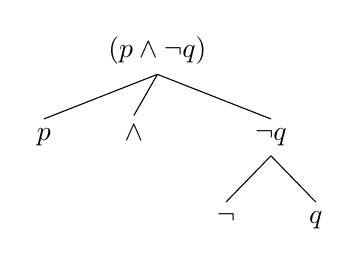
\begin{tikzpicture}[sibling distance=20pt, level distance=30pt]
    \Tree [.{$(p \wedge \neg q)$} [. $p$ ] [. $\wedge$ ] [.{$\neg q$} [. $\neg$ ] [. $q$ ] ]  ]
  \end{tikzpicture}
\end{center}

The construction of a complex formula, and therefore its syntactic tree, is always recoverable by following the introduction of the parentheses in step (iii).
This is illustrated by the minimal pair in Figure~\ref{fig:syntactic-trees}.\sidenote{This is why at most the outer parentheses may be omitted, but never any other pair of parentheses.}

\begin{figure}
  \centering

  \begin{subfigure}[b]{0.45\textwidth}
    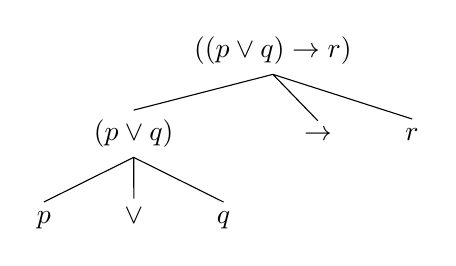
\begin{tikzpicture}[sibling distance=20pt, level distance=30pt]
      \Tree [.{$((p \vee q) \rightarrow r)$} [.{$(p \vee q)$} [. {$p$} ] [. {$\vee$} ] [. {$q$} ] ]  [. $\rightarrow$ ] [. $r$ ] ]
    \end{tikzpicture}
    \caption{Tree for $((p \vee q) \rightarrow r)$}
  \end{subfigure}
  \hfill
  \begin{subfigure}[b]{0.45\textwidth}
    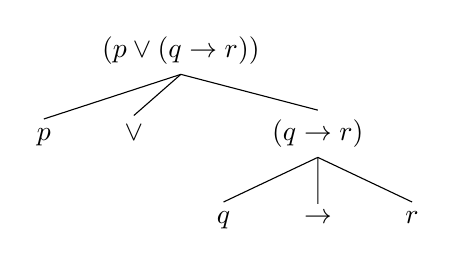
\begin{tikzpicture}[sibling distance=20pt, level distance=30pt]
      \Tree [.{$(p \vee (q \rightarrow r))$} [. $p$ ] [. $\vee$ ] [.{$(q \rightarrow r)$} [. {$q$} ] [. {$\rightarrow$} ] [. {$r$} ] ] ]
    \end{tikzpicture}
    \caption{Tree for $(p \vee (q \rightarrow r))$}
  \end{subfigure}

  \caption{Examples of syntactic trees}
  \label{fig:syntactic-trees}
\end{figure}

\subsection{Terminology}

A formula of \proplog which consist of a single proposition letter is called \emph{atomic formula.}
Any formula of \proplog which is not atomic is called a \emph{complex formula}.

Each complex formula has a \emph{main connective}.
The main connective is the last sentential connector introduced during the construction of the formula.
A complex formula is also often called by the name of its main connective.
For example, the formula $p \wedge \neg q$ has a conjunction as its main operator and would therefore be called a conjunction.
The formula $(p \vee q) \rightarrow r$ from Figure~\ref{fig:syntactic-trees}(a) is an implication, while the formula $p \vee (q \rightarrow r)$ from Figure~\ref{fig:syntactic-trees}(b) is a disjunction.

For some connectives, the subformulas that they contain may have special names as well.
In the conjunction $\varphi \wedge \psi$, the subformulas $\varphi$ and $\psi$ are called \emph{conjuncts}.
In the disjunction $\varphi \vee \psi$, the subformulas $\varphi$ and $\psi$ are called \emph{disjuncts}.
In the implication $\varphi \rightarrow \psi$, the subformula $\varphi$ is called \emph{antecedent} and the subformula $\psi$ is called \emph{consequent}.

\bigskip
\noindent \colorbox{mygray}{\centering
  \begin{minipage}{1.0\textwidth}

    \begin{exercise}
      Determine which of the following strings are formulas of propositional logic. For any formula, determine its main operator.
      \begin{multicols}{2}
        \begin{enumerate}[a.]
          \item $q_{12}$
          \item $p, q \wedge r$
          \item $(p) \wedge q$
          \item $p \rightarrow (p \wedge p)$
          \item $(p \rightarrow) (p \wedge p)$
          \item $(p \vee \neg q) \leftrightarrow (r \rightarrow (\neg (p \vee \neg p)))$
        \end{enumerate}
      \end{multicols}
    \end{exercise}

    \begin{exercise}
      Draw the syntactic tree for each of the following formulas.
      \begin{multicols}{2}
        \begin{enumerate}[a.]
          \item $p \leftrightarrow q$
          \item $\neg p \wedge p$
          \item $p \rightarrow \neg (q \wedge r)$
          \item $(\neg p \vee \neg q) \wedge (r \rightarrow p )$
        \end{enumerate}
      \end{multicols}
    \end{exercise}
  \end{minipage}
}

\newpage

\section{The semantics of propositional logic}

The language of \proplog defines rules of systematically combining proposition letters with sentential connectives.
The \emph{semantics} of \proplog gives a meaning to each formula.
Yet, \proplog is not concerned with the meaning of the proposition letters.
Whether the proposition $p$ corresponding to ``The earth is round.'' is true or false in this world we live in, is of no concern to the logician.
The (propositional) logician cares only about the meaning of the sentential connectives.
More specifically, \proplog pays attention to a specific kind of meaning, namely \emph{truth-conditional meaning}.
Concretely, \proplog analyzes the meaning of a sentential connective $\odot \in \set{\wedge,\vee,\rightarrow,\leftrightarrow}$ in terms of how the truth or falsity of the complex sentence $\varphi \odot \psi$ depends on the truth or falsity of its components $\varphi$ and $\psi$; and how the meaning of $\neg \varphi$ depends on the truth or falsity of $\varphi$.

\subsection{Truth tables}

One way of defining the semantics of the sentential connectives is by \emph{truth tables}.
Truth tables are also handy for systematically calculating the conditions under which complex formulas are true.

Take the complex formula $\neg \varphi$.\sidenote{We use $\varphi$ here as a variable which could represent any formula, no matter if it is a proposition letter or extremely long and complex.}
For all we know, $\varphi$ could be either true or false.
There are just these two possibilities.\sidenote{That \proplog only considers two truth values is also referred to as the \emph{principle of bivalence}. There are other logics, so-called many-valued logics, which allow for more than two truth values, e.g., to represent degrees of truth or uncertainty.}
To give a truth-conditional meaning to the operator $\neg$ we need to define whether $\neg \varphi$ is true or false for each case: when $\varphi$ is true, and when $\varphi$ is false.
The truth table that defines the meaning of negation is given in Table~\ref{tab:semantics-binary-connectives}(a).\sidenote{We here write 1 for the truth value ``true'' and 0 for ``false.'' It is also common to use letters $T$ and $F$, or yet other symbols in truth tables. }
\proplog treats negation like a switch: take a formula $\varphi$ as input, look at its truth value, and swap it for the other (since there are only two truth values).

Other sentential connectives than negation take two formulas as input, so to speak, and may therefore be conceived of as functions that take a pair of truth values as input to return a single truth-value.
The semantics of the binary connectives is given in Table~\ref{tab:semantics-binary-connectives}(b):

\begin{table}
  \begin{subfigure}[b]{0.3\textwidth}
    \begin{center}
      \begin{tabular}{cc}
        $\varphi$ & $\neg \varphi$ \\ \midrule
        1  & 0\\
        0  & 1
      \end{tabular}
    \end{center}
    \caption{Semantics of negation}
  \end{subfigure}
  \hfill
  \begin{subfigure}[b]{0.75\textwidth}
    \centering
    \begin{tabular}{cccccc}
      $\phi$ & $\psi$ & $\phi \wedge \psi$ & $\phi \vee \psi$ & $\phi \rightarrow \psi$ & $\phi \leftrightarrow \psi$ \\ \midrule
      1  & 1 & 1 & 1 & 1 & 1 \\
      1  & 0 & 0 & 1 & 0 & 0 \\
      0  & 1 & 0 & 1 & 1 & 0 \\
      0  & 0 & 0 & 0 & 1 & 1 \\
    \end{tabular}
    \caption{Semantics of binary connectives}
  \end{subfigure}
  \caption{Semantics of sentential connectives in propositional logic expressed in terms of truth tables}
  \label{tab:semantics-binary-connectives}
\end{table}

\subsection{Working with truth tables}

Truth tables are useful for systematically working out the conditions under which complex formulas are true.
Consider the complex formula $(\varphi \wedge \psi) \rightarrow \neg \chi$.
We do not know whether the subformula $\varphi$, $\psi$ and $\chi$ are atomic or themselves complex.
But we want to know under which truth value assignments to $\varphi$, $\psi$ and $\chi$ the formula $(\varphi \wedge \psi) \rightarrow \neg \chi$ is true or false.
In order to find out, we can construct a truth table that starts by enumerating all logical possibilities of truth-value assignments for the formulas $\varphi$, $\psi$ and $\chi$ (the first three columns in the table below).
We then work towards the ``goal formula'' $(\varphi \wedge \psi) \rightarrow \neg \chi$ by following the recursive definition of formulas of \proplog.
At each step we apply the definition of the semantics of the relevant sentential connective until we arrive at the ``goal formula''.
Following this method, we construct the truth table in Table~\ref{tab:truth-table-contingency}, which shows that the formula $(\varphi \wedge \psi) \rightarrow \neg \chi$ is always true, except when all three subformulas, $\varphi$, $\psi$ and $\chi$ are all true at the same time.

\begin{table}
  \centering
  \begin{center}
    \begin{tabular}{cccccc}
      $\varphi$ & $\psi$ & $\chi$ & $\varphi \wedge \psi$ & $\neg \chi$ & $(\varphi \wedge \psi) \rightarrow \neg \chi$ \\ \midrule
      1  & 1 & 1 & 1 & 0 & 0 \\
      1  & 1 & 0 & 1 & 1 & 1 \\
      1  & 0 & 1 & 0 & 0 & 1 \\
      1  & 0 & 0 & 0 & 1 & 1 \\
      0  & 1 & 1 & 0 & 0 & 1 \\
      0  & 1 & 0 & 0 & 1 & 1 \\
      0  & 0 & 1 & 0 & 0 & 1 \\
      0  & 0 & 0 & 0 & 1 & 1 \\
    \end{tabular}
  \end{center}

  \caption{Truth table for formula $(\varphi \wedge \psi) \rightarrow \neg \chi$}
  \label{tab:truth-table-contingency}
\end{table}

\subsection{Contingencies, tautologies \& contradictions}
\label{sec:cont-taut-}

A common application of truth tables is to find out whether a given formula is always true, always false or whether it can sometimes be true and sometimes be false.
The truth table in Table~\ref{tab:truth-table-contingency} shows that the formula $(\varphi \wedge \psi) \rightarrow \neg \chi$ belongs to the last category: there are cases, i.e., assignments of truth values to its components (= rows in the table), where it is true, and there are cases where it is false.
A formula which can become true and false for different assignments of truth values to its components is called a \emph{contingency}.
A formula which is always true under any constellation of truth values for its components is called a \emph{tautology}.
A formula which is false for all ways of assigning truth values to its subformulas is a \emph{contradiction}.
We say that a tautology is a formula that is \emph{necessarily true}, or \emph{true by logical necessity}.
Similarly, a contradiction can be said to be \emph{necessarily false}, or \emph{false by logical necessity}.\sidenote{Another way of thinking about this is to imagine that you know nothing at all about some foreign universe. You don't know at all which proposition letters are true or not. Given a tautology you can nevertheless be sure that it is true, no matter what the world is like. Of a contradiction you are sure that it is false. And for a contingency you know that you don't know whether it is true or false, before you learn facts about the world.}

To show that any formula of the form $\varphi \vee \neg \varphi$ is a tautology, we can construct the relevant truth table, shown in Table~\ref{tab:truth-tables-tautology-contradiction}(a), and check whether the column for the ``goal formula'' contains only ones, no zeros.
Similarly, the truth table in Table~\ref{tab:truth-tables-tautology-contradiction}(b) reveals that any formula of the logical form $\varphi \wedge \neg \varphi$ is a contradiction.

\begin{table}
  \begin{subfigure}[b]{0.45\textwidth}
    \centering
    \begin{tabular}{cc>{\columncolor{olive!15}}c}
      $\varphi$ & $\neg \varphi$ & $\varphi \vee \neg \varphi$ \\ \midrule
      1  & 0 & 1\\
      0  & 1 & 1
    \end{tabular}
    \caption{Truth table for $\varphi \vee \neg \varphi$}
    \label{tab:truth-table-tautology}
  \end{subfigure}
  \hfill
  \begin{subfigure}[b]{0.45\textwidth}
    \centering
    \begin{tabular}{cc>{\columncolor{olive!15}}c}
        $\varphi$ & $\neg \varphi$ & $\varphi \wedge \neg \varphi$ \\ \midrule
        1  & 0 & 0\\
        0  & 1 & 0
      \end{tabular}
    \caption{Truth table for $\varphi \wedge \neg \varphi$}
    \label{tab:truth-table-contradiction}
  \end{subfigure}
  \caption{Truth tables for a tautology and a contradiction}
  \label{tab:truth-tables-tautology-contradiction}
\end{table}

\subsection{Logical equivalence}

Two formulas $\varphi$ and $\psi$ are logically equivalent if they have exactly the same truth value no matter how we assign meanings to all subformulas of $\varphi$ and $\psi$, as long as we assign any subformula that occurs in both $\varphi$ and $\psi$ the same truth value.
We can use truth table to test when or demonstrate that two formulas are logically equivalent.
To do this, we just have to make a combined truth table in which we have one column for $\varphi$ and another for $\psi$.
$\varphi$ and $\psi$ are logically equivalent exactly when the truth values in the columns that correspond to them are identical in each row.
The truth table in Table~\ref{tab:truth-table-equivalence} shows that $\varphi \wedge \neg \psi$ and $\neg (\varphi \rightarrow \psi)$ are in fact logically equivalent.

\begin{table}
  \centering
  \begin{center}
    \begin{tabular}{ccc>{\columncolor{olive!15}}cc>{\columncolor{olive!15}}c}
      $\varphi$ & $\psi$ & $\neg \psi$ & $\varphi \wedge \neg \psi$ & $\varphi \rightarrow \psi$ & $\neg (\varphi \rightarrow \psi)$ \\ \midrule
      1  & 1 & 0 & 0 & 1 & 0 \\
      1  & 0 & 1 & 1 & 0 & 1 \\
      0  & 1 & 0 & 0 & 1 & 0 \\
      0  & 0 & 1 & 0 & 1 & 0 \\
    \end{tabular}
  \end{center}

  \caption{Truth table showing the equivalence of $\varphi \wedge \neg \psi$ and $\neg (\varphi \rightarrow \psi)$}
  \label{tab:truth-table-equivalence}
\end{table}

If two formulas $\varphi$ and $\psi$ are \emph{not} logically equivalent, we can also show this with a truth table.
In that case, there must be at least one row in which their truth values differ.
In practice it may help to mark one such row as the refuting counterexample against the assumption of logical equivalence.
This is shown in Table~\ref{tab:truth-table-}.

\begin{table}
  \centering
  \begin{center}
    \begin{tabular}{cc>{\columncolor{olive!15}}c>{\columncolor{olive!15}}cc}
      $\varphi$ & $\psi$ & $\varphi \rightarrow \psi$ & $\varphi \leftrightarrow \psi$ & counterexample \\ \midrule
      1  & 1 & 1 & 1 \\
      1  & 0 & 0 & 0 \\
      0  & 1 & 1 & 0 & $\Leftarrow$\\
      0  & 0 & 1 & 1 \\
    \end{tabular}
  \end{center}

  \caption{Truth table showing the non-equivalence of $\varphi \rightarrow \psi$ and $\varphi \leftrightarrow \psi$}
  \label{tab:truth-table-}
\end{table}


%%%%%%%%%%%%%%%%%%%%%%%%%%%%%%%%%%%%%%%%%%%%%%%%%%

\bigskip
\noindent \colorbox{mygray}{\centering
  \begin{minipage}{1.0\textwidth}

    \begin{exercise}
      For each of the following formulas, try to intuit whether it is a tautology, a contradiction or a contingency. Write down your best guess. Then use the truth-table method to find out for certain.
      \begin{multicols}{2}
        \begin{enumerate}[a.]
          \item $\varphi \rightarrow \neg \varphi$
          \item $\varphi \leftrightarrow (\varphi \wedge \psi)$
          \item $(\varphi \wedge \neg \varphi) \rightarrow \psi$
          \item $(\varphi \wedge \neg \psi) \leftrightarrow (\varphi \rightarrow \psi)$
        \end{enumerate}
      \end{multicols}
    \end{exercise}

    \begin{exercise}
      For each of the following pairs of formulas, try to intuit whether they are logically equivalent of not. Write down you guess. Then use truth tables to determine whether they are. Highlight the relevant columns in your truth table. Mark a row as a counterexample if they are not.
      \begin{multicols}{2}
        \begin{enumerate}[a.]
          \item $\varphi$, \ $\neg \neg \varphi$
          \item $\varphi \leftrightarrow \phi$, \ $\varphi \wedge \psi$
          \item $\neg \varphi \vee  \psi$, \  $\varphi \rightarrow \psi$
          \item $\varphi \vee (\chi \rightarrow \neg \varphi)$, \ $\psi \vee (\chi \rightarrow \neg \psi)$
        \end{enumerate}
      \end{multicols}
    \end{exercise}

  \end{minipage}
}

\newpage

\section{Logical structure of meaning}
\label{sec:excav-prop-logic}

Linguistic theory distinguishes between \emph{semantic meaning} of a sentence or an expression and additional \emph{pragmatic enrichments} to the literal meaning.
The literal meaning is the context-independent logical core meaning.
Pragmatic enrichments arise in context by taking into account general world knowledge or the reasons why a speaker used language in the way that they did.
Pragmatic enrichments may be part of what we ``perceive'' to be the most likely interpretation of a sentence; they may be what the speaker meant to say, but not what the sentence means literally.\sidenote{The most obvious example is an utterance of a sentence like \emph{The weather is so nice today!} when clearly meant ironically.}

Our current goal is to learn to excavate the logical structure of natural language sentences.
Therefore, we have to learn to ``strip off the pragmatic layer,'' so to speak.
Indeed, the logical operators of \proplog bear a close correspondence to natural language expressions \emph{and}, \emph{or}, \emph{if} and \emph{if and only if}.
But the correspondence is not a perfect match.
This is partly due to the difference between semantic meaning and pragmatic enrichment.\sidenote{There are also arguments suggesting that the logical operators of \proplog are \emph{not} good enough for analyzing the semantic meaning of their corresponding natural language expressions. Most importantly, this concerns the semantic meaning of conditional sentences, i.e., natural language sentences with \emph{if dots, then \dots}.}
Let us look at a few interesting cases.

\subsection{Conjunction \& order-sensitivity}

Logical conjunction is order-insensitive: $\varphi \wedge \psi$ and $\psi \wedge \varphi$ are logically equivalent.
But natural language conjunctions are not necessarily.
Saying that
\begin{quote}
  \textit{They got married and had children.}
\end{quote}
might be understood differently from saying that
\begin{quote}
  \textit{They had children and got married.}
\end{quote}
Still, we would analyze both of these sentences as having a logical-conjunctive meaning,
additional inferences about the temporal order of events notwithstanding.

\subsection{Disjunction: inclusive vs.~exclusive}

Logical disjunction is \emph{inclusive}: $\varphi \vee \psi$ is true when $\varphi$ and $\psi$ are both true.
Yet natural language disjunctions \emph{can} be understood as exclusive disjunction according to which exactly one, but not both disjuncts are true.
For example, if I say:
\begin{quote}
 \textit{She owns a Porsche or a Ferrari.}
\end{quote}
you might take that to mean that she doesn't own both.
But did I \emph{literally} say that?
--- The logical meaning of that sentence is more plausibly just analyzed as inclusive disjunction.
This is because it is not contradictory to say:
\begin{quote}
 \textit{She owns a Porsche or a Ferrari and possibly both.}
\end{quote}
This contrasts with the weirdness of saying:
\begin{quote}
 \textit{She owns \emph{either} a Porsche or a Ferrari and possibly both.}
\end{quote}
suggesting that natural language \emph{either \dots or \dots} \emph{does} have an exclusive disjunctive meaning, but simple \emph{or} does not.

\subsection{Conditional perfection}

\proplog analyzes implication as so-called \emph{material implication}, but it is controversial whether natural language conditional sentences might not have a much richer meaning, e.g., requiring a discernible causal-inferential relation between antecedent and consequent.
Moreover, similar to the case of inclusive vs.~exclusive disjunctions, many natural language conditionals receive a so-called \emph{conditional perfection reading}, i.e., they are read like an ``if and only if'' statement which would correspond to logical operator $\leftrightarrow$, even though their logical meaning might just be that of a simple implication $\rightarrow$.
For example, the conditional statement:
\begin{quote}
 \textit{If Bubu comes, Kiki comes.}
\end{quote}
does suggest to a certain degree that Kiki \emph{only} comes when Bubu does.
But that is not the logical core meaning of this sentence, but rather a pragmatic enrichment on top of the logical meaning of the sentence.
To see this, compare the difference in weirdness between saying
\begin{quote}
 \textit{If Bubu comes, Kiki comes, and maybe Kiki comes no matter what.}
\end{quote}
which seems fine, especially when compared to the much weirder:
\begin{quote}
 \textit{Kiki comes only if Bubu comes, and maybe Kiki comes not matter what.}
\end{quote}

\subsection{Excavating the logical structure of natural language sentences}

Despite superficial discrepancies, it is possible and highly informative to try to lay bare the logical structure of natural language sentences.% \sidenote{There are least two attitudes you can adopt to approach this endeavour. You can think that there \emph{is} a true logical structure to be found, so that, if you struggle or find mismatches, it must mean that you are learning something about the nature of the true underlying logic. Or you can realize that trying to find the logical structure, even though you do not believe that there is single true one, is informative because it tells you something about the limits of logic and the aspects of natural language which cannot (easily) be captured by logical analysis (of the kind we use here).}
The logical relation between propositions contained in a natural language sentence may sometimes be opaque.
Take the following example sentence:
\begin{quote}
  \emph{If drawing a red card means that I lost, I lost.}
\end{quote}
This sentences does have a propositional-logical structure, even though it is not at all apparent from the way it is realized in natural language.
There are two atomic (truth-evaluable) propositions involved here:
\begin{multicols}{2}
  \begin{itemize}[]
    \item $p$: I drew a red card.
    \item $q$: I lost.
  \end{itemize}
\end{multicols}
\noindent With this \emph{translation key}, we can then determine the logical structure of the sentence above as:
\begin{align*}
  (p \rightarrow q) \rightarrow q
\end{align*}

Here are a few other examples.
\begin{enumerate}[(i)]
  \item John is hungry. \\
    \emph{Key:} $p$: John is hungry. \ \ \ \ \ \
    \emph{Logical form:} $p$

  \item Mary likes John.\\
      \emph{Key:} $p$: Mary likes John. \ \ \ \ \
      \emph{Logical form:} $p$

  \item John is hungry and Mary likes John.\\
        \emph{Key:}
          $p$: John is hungry. \ \ \ \ \
          $q$: Mary likes John. \\
        \emph{Logical form:} $p \wedge q$

  \item Berlin is east of Hamburg and Bremen.\\
        \emph{Key:}
        $p$: Berlin is east of Hamburg. \ \ \ \ \
        $q$: Berlin is east of Bremen.\\
        \emph{Logical form:} $p \wedge q$

  \item Call me `sweetie' once more and, no kidding, I'll step on your toe.\\
        \emph{Key:}
        $p$: I'm not kidding. \ \ \ \
        $q$: I'll step on your toe. \\
        \textcolor{white}{\emph{Key:}} $r$: You call me `sweetie' once more.\\
        \emph{Logical form:} $p \wedge (r \rightarrow q)$

  \item  I will only play salsa, if you give me earplugs.\sidenote{There is a likely inclination to analyze this as $p \leftrightarrow q$, but it is not clear whether this is part of the semantic/logical content here. Suppose you know that the sentence is true. Now you learn that earplugs have been handed over. Does that \emph{logically} entail that salsa was played? No, because the sentence only says that earplugs are a \emph{necessary} but not necessarily \emph{sufficient} condition for salsa.}\\
        \emph{Key:}
                $p$: I will play salsa. \ \ \ \ \
                $q$: You give me earplugs.\\
        \emph{Logical form:} $p \rightarrow q$
\end{enumerate}

\bigskip
\noindent \colorbox{mygray}{\centering
  \begin{minipage}{1.0\textwidth}

    \begin{exercise}
      For each of the following sentences give the translation key and the (propositional) logical form.
      \begin{enumerate}[(a.)]
        \item If John is hungry, then Mary likes John.
        \item If John is hungry and Bill runs, then Mary doesn't likes John.
        \item John is hungry or it's false that Bill runs.
        \item Mary likes John or Mary doesn't like John.
        \item Mary likes John but John is hungry.
        \item Mary likes John provided Bill runs.
      \end{enumerate}
    \end{exercise}

  \end{minipage}
}

\newpage

\section{Valuation functions, possible worlds \& logical entailment}

\subsection{Valuation functions}

The truth-tables method introduced above is very practical, but a proper definition of the semantics of \proplog should better not rely on vocabulary like ``rows'' and ``columns,'' but use mathematical notions like ``function'' or ``set.''
The proper definition of the semantics of \proplog is therefore formulated in terms of so-called valuation functions.

A \emph{valuation function} $V$ is a function that assigns to every formula of propositional logic a unique truth value (0 or 1).
More specifically, think of a valuation function as a way of assigning truth-values to all proposition letters.
Once we know the truth or falsity of all proposition letters, the truth or falsity of all complex formulas is non-arbitrary, because it is fixed by the meaning of the sentential connectives.

\begin{table}
  \centering
  \begin{tabular}{lcl}
    $V(p)$, $V(q)$, \dots && arbitrary\\
    $V(\neg \phi) = 1$ & iff & $V(\phi) =0$\\
    $V(\phi \wedge \psi) = 1$ & iff & $V(\phi) =1$ and $V(\psi) = 1$\\
    $V(\phi \vee \psi) = 1$ & iff & $V(\phi) =1$ or $V(\psi) = 1$\\
    $V(\phi \rightarrow \psi) = 0$ & iff & $V(\phi) =1$ and $V(\psi) = 0$\\
    $V(\phi \leftrightarrow \psi) = 1$ & iff & $V(\phi) = V(\psi)$
  \end{tabular}
  \caption{Semantics of propositional logic in terms of valuation functions}
  \label{tab:proplog-semantics-valuation-functions}
\end{table}

A valuation function is analogous to a row in a truth table, when we use proposition letters, not variables for formulas like $\varphi$ or \(\psi\).\sidenote{If we use truth tables for complex formulas built with Greek letters like $\varphi$ or $\psi$, we cannot say that a row corresponds to a valuation function because we do not know what the variables like $\varphi$ or \(\psi\) represent. For example, $\varphi$ might be a tautology or a contradiction. We would still write out all possible truth-value assignments for $\varphi$, but we just cannot be sure if there is a valuation function that would correspond to each row. For this reason, when we look at argument schemas below, using truth tables to check for logical validity, we use proposition letters instead of variables for formulas.}

\subsection{Possible worlds \& truth-conditional meaning}

A valuation function can also be thought of as a \emph{possible world}.\sidenote{This terminology is widely used in formal semantics and philosophy.}
A possible world is a way in which things could be.
A possible world conforms to the rules of logic, but otherwise allows all atomic propositions to be different from the facts in the \emph{actual world}.

Using valuation functions or, equivalently, possible worlds, we can give a clear definition of the meaning of a formula (and, therefore by extension, to the logical meaning of a natural language sentence).
The truth-conditional meaning of formula $\varphi$ is the set of all valuation functions, or possible worlds, for which $\varphi$ is true.
Formal semantics often uses notation $\den{\varphi}$ to denote the meaning of a formula in this sense:
\begin{align*}
  \den{\varphi} = \set{V \mid V \text{ is a valuation function such that } V(\varphi)=1 }
\end{align*}
Alternatively, we could say that the meaning of a formula is the set of possible worlds in which it is true.\sidenote{Compare the famous passage from Wittgenstein's \emph{Tractatus Logica Philosophicus}: ``Einen Satz verstehen, heißt, wissen was der Fall ist, wenn er wahr ist.
(Man kann ihn also verstehen, ohne zu wissen, ob er wahr ist.)'' [TLP 4.024]
}

\subsection{Tautologies, contradictions, contingencies \& equivalence (revisited)}

Using valuation functions and/or possible worlds, we can also give a proper definition of notions we used previously in the context of truth tables.
We say that $\varphi$ is a tautology iff $V(\varphi) = 1$ for all valuation functions $V$.
We say that $\varphi$ is a contradiction iff $V(\varphi) = 0$ for all valuation functions $V$.
We say that $\varphi$ is a contingency iff there is at least one valuation function $V_{1}$ such that $V_{1}(\varphi) = 1$ and there is at least one valuation function $V_{2}$ such that $V_{2}(\varphi) = 0$.
We say that $\varphi$ and \(\psi\) are logically equivalent, iff for all valuation functions $V(\varphi) = V(\psi)$.


\subsection{Logical entailment \& informativity}

Similarly, we can now give a proper definition of logical entailment.
Formula $\varphi$ logically entails $\psi$ iff for all valuation functions $V$, if $V(\varphi)=1$, then $V(\psi)=1$.
An alternative formulation is this: $\varphi$ logically entails $\psi$ iff $\den{\varphi} \subseteq \den{\psi}$.

Based on the notion of logical meaning in terms of sets of possible worlds, we can also tackle another otherwise extremely elusive concept, namely that of \emph{informativity}, i.e., the amount of information given.
We say that $\varphi$ is at least as informative as $\psi$ iff $\den{\varphi} \subseteq \den{\psi}$, and that $\varphi$ is strictly more informative than $\psi$ iff $\den{\varphi} \subset \den{\psi}$.

This notion of logical informativity is a relative one.
It does not give an absolute measure of information for each formula, but only compares two formulas in terms of their relative informativity.
It also only compares some formulas; in fact, the ordering induced by this definition of logical informativity is a \emph{partial order}.\sidenote{Probabilistic notions of information, e.g., as given by information-theory extend the notion of logical information to an absolute measure of information which yields a total order.}

\subsection{Argument schemas \& validity}

The important concept of logical validity can be thought, at least for \proplog, of as an extension of the notion of logical entailment to more than two formulas.
Concretely, we defined logical validity of so-called argument schemas.
If $\varphi_1, \varphi_2, \dots, \varphi_n$ and $\psi$ are forumlas of propositional logic, then $\varphi_1, \varphi_2, \dots, \varphi_n / \psi$ is an \markdef{argument schema}.
Formulas $\varphi_1, \varphi_2, \dots, \varphi_n$ are the \markdef{premisses}, formula $\psi$ is the \markdef{conclusion}.

The argument schema $\varphi_1, \varphi_2, \dots, \varphi_n / \psi$ is \markdef{valid} iff for all
valuation functions $V$ such that $V(\varphi_1)=V(\varphi_2)= \dots = V(\varphi_n)=1$ it also holds
that $V(\psi) = 1$.
If valid, we write $\varphi_1, \varphi_2, \dots, \varphi_n \models \psi$.

We can use truth tables again to check whether any given argument schema is valid or not.
Consider the argument schema: $p \vee q$, $\neg q$ / $p$.
A natural language analogue would be the following.
We know or assume the following premisses:
\begin{quote}
  The murderer is the butler or the gardener. \\
  The gardener is not the murderer.
\end{quote}
And the putative conclusion is:
\begin{quote}
  The butler is the murderer.
\end{quote}
We would like to find out whether the conclusion logically follows from the premisses.
Table~\ref{tab:truth-table-valid} tells us that it does: in all rows (=valuation functions or possible worlds) in which all the premisses are true, which are marked with an asterisk (*) in Table~\ref{tab:truth-table-valid}, the conclusion (in the last column) is also true.

\begin{table}
  \centering
  \begin{tabular}{cccccc}
    $p$ & $q$ & $p \vee q$ & $\neg q$ & / & $q$ \\ \midrule
    1  & 1 & 1 & 0 &   & 1  \\
    1  & 0 & 1 & 1 & * & 1  \\
    0  & 1 & 1 & 0 &   & 0  \\
    0  & 0 & 0 & 1 &   & 0  \\
  \end{tabular}
  \caption{Truth table for checking the validity of argument schema}
  \label{tab:truth-table-valid}
\end{table}

Table~\ref{tab:arg-schema-invalid} shows a more extensive example of the truth-table method for the argument schema  $\neg p \rightarrow (q \wedge \neg r)$, $\neg q \rightarrow \neg r$ / $p$, which is not valid.
The table also introduces names for each row, in terms of (types of) possible worlds, so that we can conveniently say that a possible world like $w_{6}$ in which $p$ and $r$ are false and $q$ is true is a counterexample to validity: both premises are true, but the conclusion is false.

\begin{table*}
  \centering
  \begin{tabular}{ccccccc>{\columncolor{olive!15}}cc>{\columncolor{olive!15}}cc>{\columncolor{olive!15}}ccl}
    & $p$ & $q$ & $r$ & $\neg p$ & $\neg r$ & $q \wedge \neg r$
    & $\neg p \rightarrow (q \wedge \neg r)$ & $\neg q$
    & $\neg q \rightarrow \neg r$ & $/$ & $p$ & \\ \midrule
    $w_{1}$ & 1  & 1 & 1 & 0 & 0 & 0 & 1 & 0 & 1 & * & 1  & \\
    $w_{2}$ & 1  & 1 & 0 & 0 & 1 & 1 & 1 & 0 & 1 & * & 1  & \\
    $w_{3}$ & 1  & 0 & 1 & 0 & 0 & 0 & 1 & 1 & 0 &   & 1  & \\
    $w_{4}$ & 1  & 0 & 0 & 0 & 1 & 0 & 1 & 1 & 1 & * & 1  & \\
    $w_{5}$ & 0  & 1 & 1 & 1 & 0 & 0 & 0 & 0 & 1 &   & 0  & \\
    $w_{6}$ & 0  & 1 & 0 & 1 & 1 & 1 & 1 & 0 & 1 & * & 0  & $\leftarrow$\\
    $w_{7}$ & 0  & 0 & 1 & 1 & 0 & 0 & 0 & 1 & 0 &   & 0  & \\
    $w_{8}$ & 0  & 0 & 0 & 1 & 1 & 0 & 0 & 1 & 1 &   & 0  & \\
  \end{tabular}
  \caption{Example of the truth-table method applied to an argument schema that is not valid}
  \label{tab:arg-schema-invalid}
\end{table*}

\subsection{Theorems of propositional logic}

Based on the definitions we have seen so far, we can make prove illuminating facts about \proplog.
Here are some examples.

\begin{proposition}
 If $\varphi$ is a tautology, then $\neg \varphi$ is a contradiction.
\end{proposition}

\begin{proof}
  If $\varphi$ is a tautology, then for all valuation functions $V$ we have $V(\varphi) = 1$. For any valuation function $V$ if $V(\varphi) = 1$, by definition also $V(\neg \varphi) = 0$. Therefore, $V(\neg \varphi) = 0$ for all $V$, which means that $\varphi$ is a contradiction.
\end{proof}

\begin{proposition}
 $\varphi \rightarrow \psi$ is a tautology iff $\varphi$ logically entails $\psi$.\sidenote{Notice that this may seem trivial, but there are really two notions that are related by this proposition. One is the definition of the sentential connective $\rightarrow$, the other is a high-level notion of logical entailment defined on top of the semantics for \emph{all} formulas.}
\end{proposition}

\begin{proof}
  First assume that $\varphi \rightarrow \psi$ is a tautology. We need to show that it follows that $\varphi$ logically entails $\psi$. Towards contradiction, let us assume that $\varphi$ does not logically entail $\psi$. This can only be the case if there is at least one valuation function $V$ for which $V(\varphi) = 1$ and $V(\psi) = 0$. For this valuation function, by definition of the meaning of $\rightarrow$, it holds that $V(\varphi \rightarrow \psi)=0$. So, we contradict our assumption that $\varphi \rightarrow \psi$ is a tautology. \\
  Next, we assume that $\varphi$ logically entails $\psi$. We need to show that $\varphi \rightarrow \psi$ is a tautology. If $\varphi$ logically entails $\psi$, this means that there is no valuation function $V$ for which $V(\varphi)=1$ and $V(\psi)=0$. But, from the definition of the semantics of $\rightarrow$, we know that the only possibility for $\varphi \rightarrow \psi$ to be false is if $V(\varphi)=1$ and $V(\psi)=0$. Since this is ruled out by our assumption, $\varphi \rightarrow \psi$ must be a tautology.
\end{proof}

\bigskip
\noindent \colorbox{mygray}{\centering
  \begin{minipage}{1.0\textwidth}

    \begin{exercise}
      Use the truth-table method to check whether the following argument schemas are valid:
      \begin{enumerate}[(i)]
        \item $p \rightarrow q$, $p$ / $q$ \hfill [\mygray{modus ponens}]
        \item $p \rightarrow q$, $q$ / $p$ \hfill [\mygray{affirmation of the consequent}]
        \item $p \rightarrow q$, $\neg q$/ $\neg p$ \hfill [\mygray{modus tollens}]
        \item $\neg(p \wedge q)$, $\neg q$ / $p$
      \end{enumerate}
    \end{exercise}

    \begin{exercise}
      For each of the following claims, determine whether it is true or false. If it is true prove it. If it is false, give a refutation by counterexample.
      \begin{enumerate}[(i)]
        \item If $\varphi$ is a tautology and $\psi$ is a contradiction,  $\varphi \rightarrow \psi$ is a contradiction.
        \item If $\psi$ is a tautology,  $\varphi \rightarrow \psi$ is a tautology.
        \item If $\varphi$ is a tautology,  $\varphi \rightarrow \psi$ is a tautology.
        \item If $\varphi \vee \psi$ is a contradiction,  $\varphi$ is a contradiction.
      \end{enumerate}
    \end{exercise}
  \end{minipage}
}

\end{document}

information
